% !TEX TS-program = pdfLaTeX+shellescape
% !TEX encoding = UTF-8 Unicode

\documentclass[class=beamer,tikz]{standalone}
\setbeamertemplate{navigation symbols}{} % For delete the navigation symbols
\usefonttheme{professionalfonts}
\usepackage{luatexja}
% \usepackage{pgfplots}
% \pgfplotsset{compat=1.17}

\usepackage{colortbl,array,xcolor}
\usepackage{amsmath,amsfonts}

\begin{document}
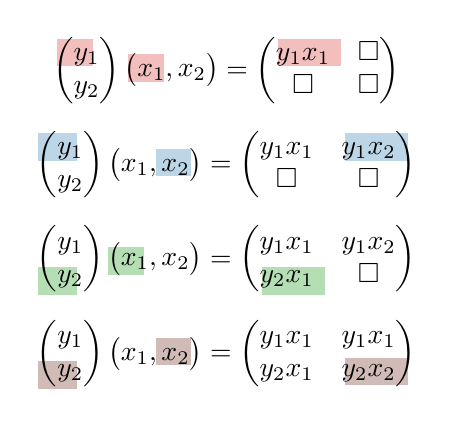
\begin{tikzpicture}
    \definecolor{tab_red}{HTML}{d62728}
    \definecolor{tab_blue}{HTML}{1f77b4}
    \definecolor{tab_green}{HTML}{2ca02c}
    \definecolor{tab_yellow}{HTML}{8c564b}
    %\draw[help lines] (0,0) grid (12,5.2);
    \path[fill=tab_red!30] (3.85,4.65) rectangle (4.30,5.00);
    \path[fill=tab_red!30] (4.75,4.45) rectangle (5.20,4.80);
    \path[fill=tab_red!30] (6.65,4.65) rectangle (7.45,5.00);
    \path[fill=tab_blue!30] (3.60,3.45) rectangle (4.10,3.80);
    \path[fill=tab_blue!30] (5.10,3.25) rectangle (5.55,3.60);
    \path[fill=tab_blue!30] (7.50,3.45) rectangle (8.30,3.80);
    \path[fill=tab_green!35] (3.60,1.75) rectangle (4.10,2.10);
    \path[fill=tab_green!35] (4.50,2.00) rectangle (4.95,2.35);
    \path[fill=tab_green!35] (6.45,1.75) rectangle (7.25,2.10);
    \path[fill=tab_yellow!40] (3.60,0.55) rectangle (4.10,0.90);
    \path[fill=tab_yellow!40] (5.10,0.85) rectangle (5.55,1.20);
    \path[fill=tab_yellow!40] (7.50,0.60) rectangle (8.30,0.95);
    
    \node (matrix0) at (6.0,4.6) {
        $\begin{pmatrix}
            y_1 \cr y_2
        \end{pmatrix}\begin{pmatrix}
            x_1, x_2
        \end{pmatrix} = \begin{pmatrix}
            y_1x_1 & \square \cr 
            \square & \square 
        \end{pmatrix}$
    };
    \node (matrix1) at (6.0,3.4) {
        $\begin{pmatrix}
            y_1 \cr y_2
        \end{pmatrix}\begin{pmatrix}
            x_1, x_2
        \end{pmatrix} = \begin{pmatrix}
            y_1x_1 & y_1x_2 \cr 
            \square & \square 
        \end{pmatrix}$
    };
    \node (matrix2) at (6.0,2.2) {
        $\begin{pmatrix}
            y_1 \cr y_2
        \end{pmatrix}\begin{pmatrix}
            x_1, x_2
        \end{pmatrix} = \begin{pmatrix}
            y_1x_1 & y_1x_2 \cr 
            y_2x_1 & \square 
        \end{pmatrix}$
    };
    \node (matrix3) at (6.0,1) {
        $\begin{pmatrix}
            y_1 \cr y_2
        \end{pmatrix}\begin{pmatrix}
            x_1, x_2
        \end{pmatrix} = \begin{pmatrix}
            y_1x_1 & y_1x_1 \cr 
            y_2x_1 & y_2x_2 
        \end{pmatrix}$
    };
\end{tikzpicture}
\end{document}